\documentclass[dvipdfmx,fleqn]{beamer}
%\documentclass[dvipdfmx,fleqn,handout]{beamer}
\usepackage{amsmath,amssymb,amsthm}

\mode<presentation>
{
  \usetheme{default}
}

\title{\Large タイトル}
\author{\large 名前}
\date{\small 日付}

\usefonttheme{professionalfonts}

\setbeamercovered{transparent=20}

\setbeamertemplate{navigation symbols}{} 
\setbeamertemplate{footline}[frame number] 



\begin{document}

\sffamily
\gtfamily


\begin{frame}
  \titlepage
  \thispagestyle{empty}
\end{frame}

\setcounter{framenumber}{0}




\begin{frame}
\frametitle{はじめに}
\begin{itemize}\setlength{\parskip}{0.5em}
\item
項目1

\item
項目2
 \begin{itemize}\setlength{\parskip}{0.5em}
 \item
 1階層下の項目1
 \item
 1階層下の項目2
 \end{itemize}

\item
このページの最後の項目
\end{itemize}
\end{frame}



\begin{frame}
\frametitle{次のスライド}
\begin{itemize}\setlength{\parskip}{0.5em}
\item
Ficititious playの説明1

\item
Ficititious playの説明2 \pause

$x_0(t)$ は
\[
x_0(t+1)
= x_0(t) + \frac{1}{t+2} (a_1(t) - x_0(t))
\]
と再帰的に書くことができる. \pause

\item
Ficititious playの説明3 \pause

\item
``\texttt{pause}''をつけるとoverlayができる.

\item
ファイルの冒頭の\texttt{documentclass}のオプションで\texttt{handout}を指定すると,
overlayにならずいっぺんに表示される.

Webにのせるときや,印刷して配るときなどは\texttt{handout}を指定しておく.

\end{itemize}
\end{frame}



\begin{frame}[fragile]   %[containsverbatim]% verbatim 環境を使えるように
\frametitle{コードの説明}
\begin{itemize}\setlength{\parskip}{0.5em}
\item
ライブラリのインポートとクラスの定義 \pause
\scriptsize
\begin{verbatim}
import matplotlib.pyplot as plt
import random
import numpy as np


\end{verbatim}
\pause
\normalsize
\item
matplotlib.pyplotはグラフのプロットに使用 \pause

\item
randomは初期信念と行動を定めるのに使用 \pause

\item
numpyは行列計算に使用


\end{itemize}
\end{frame}

\begin{frame}[fragile]% verbatim 環境を使えるように
\frametitle{コードの説明とか}
\begin{itemize}\setlength{\parskip}{0.5em}
\item

\scriptsize
\begin{verbatim}
class FP:

    def __init__(self, profits):
        self.pro = profits
        self.cu_xs = [0, 0]
        self.x0s = []
        self.x1s = []
 
 \end{verbatim}
\normalsize

\item
いくつかのメソッドをもつクラスをFPとして定義\pause
\item
FPを使う際にはf = FP(profits)のように打つ必要がある\pause
\item
profitsは利得表を表す行列である\pause
\item
initメソッド中でインスタンス変数をいくつか定義している \pause
これはクラス内でのみ共有される \pause
複数のメソッドで用いる変数をここに記した



\end{itemize}
\end{frame}
 
\begin{frame}[containsverbatim]% verbatim 環境を使えるように
\frametitle{コードの説明とか}
\begin{itemize}\setlength{\parskip}{0.5em}
\item
コードの表示の例
\scriptsize
\begin{verbatim}
    def oneplay(self, ts_length):
        pro_cal = (np.transpose(self.pro)[0],
                   np.transpose(np.transpose(self.pro)[1]))
        self.x0s = []
        self.x1s = []
        self.cu_xs = [random.uniform(0, 1), random.uniform(0, 1)]
        cu_es = [[0, 0], [0, 0]]
        for i in range(ts_length):
            self.x0s.append(self.cu_xs[0])
            self.x1s.append(self.cu_xs[1])
            exp = ((1-self.cu_xs[0], self.cu_xs[0]),
                   (1-self.cu_xs[1], self.cu_xs[1]))
            cu_es[0] = np.dot(pro_cal[0], exp[0])
            cu_es[1] = np.dot(pro_cal[1], exp[1])
            cu_as = [0, 0]  # the act of players
            for j in range(2):
                if cu_es[j][0] == cu_es[j][1]:
                    cu_as[j] = random.randint(0, 1)
                else:
                    cu_as[j] = cu_es[j].argmax()
            for k in range(2):
                self.cu_xs[k] = (self.cu_xs[k]*(i+1)+cu_as[1-k])/(i+2)
                # x(i) to x(i+1)

    def playplot(self, ts_length):
        self.oneplay(ts_length)
        plt.plot(self.x0s, 'b-', label='x_0(t)')
        plt.plot(self.x1s, 'r-', label='x_1(t)')
        plt.legend()
        plt.show()

    def playsave(self, ts_length, name):  # name is str
        self.oneplay(ts_length)
        plt.plot(self.x0s, 'b-', label='x_0(t)')
        plt.plot(self.x1s, 'r-', label='x_1(t)')
        plt.legend()
        plt.savefig(str(name)+'.png', bbox_inches='tight', pad_inches=0)
        plt.savefig(str(name)+'.pdf', bbox_inches='tight', pad_inches=0)
        plt.close()

    def histogram(self, n, ts_length):
        last_x0s = []
        for j in range(n):
            self.oneplay(ts_length)
            last_x0s.append(self.cu_xs[0])
        ax = plt.subplot(111)
        ax.hist(last_x0s, alpha=0.6, bins=5)
        ax.set_xlim(xmin=0, xmax=1)
        t = 'ts = '+str(ts_length)+', times = '+str(n)
        ax.set_title(t)

    def histplot(self, n, ts_length):
        self.histogram(n, ts_length)
        plt.show()

    def histsave(self, n, ts_length, name):
        self.histogram(n, ts_length)
        plt.savefig(str(name)+'.png', bbox_inches='tight', pad_inches=0)
        plt.savefig(str(name)+'.pdf', bbox_inches='tight', pad_inches=0)
        plt.close()

\end{verbatim}

\item
\verb|\begin{frame}| から \verb|\end{frame}| までを
コピー\&ペーストしてスライドを増やしていく.
\end{itemize}
\end{frame}



\begin{frame}
\frametitle{図}
\begin{figure}
 \centering
 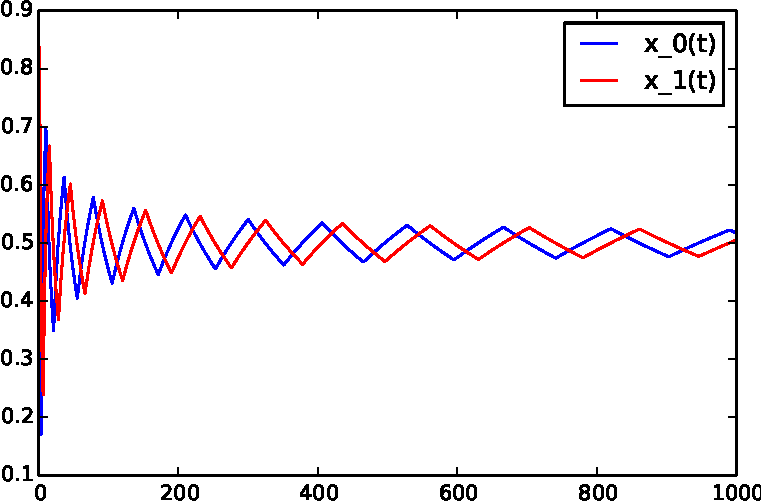
\includegraphics[width=\linewidth]{oneplay2.pdf}
 \caption{図の表示}
 \label{fig:matchingpennies_plot}
\end{figure}
\end{frame}



\begin{frame}
\frametitle{まとめ}
\begin{itemize}\setlength{\parskip}{0.5em}
\item
まとめ

\item
よくわかっていない点とか

\item
今後の課題とか
\end{itemize}
\end{frame}



\end{document}